\section{EBNF Notation}
Besides basic BNF support, gt also supports context-free grammars with EBNF notation. A user is able to define a 
production that has optional and repetitive types. The optional type allows an element(s) to have one or none and
the repetitve feature allows element(s) to be zero or many, one or many or n or many
where n is a non-negative integer. With the repetitive types a user can also define 
whether it is left or right associative.  Gt's syntax for EBNF notation is explained below.

% EBNF Simple example
\subsection{Example - Simple}
The following is a very basic grammar definition for gt. When completed the 
grammar will allow for one to many ID's where each is separated by a PLUS (eg. x + x). 
This example can be found in \textit{gt/tests/bnf/simple.gra}. 

First, a name for your grammar will need to be defined. A grammar name is the first declaration in a gt
definition. It starts with a lowercase letter that is followed
by zero or many upper- or lowercase letters, underscores and/or numbers (['a'-'z' 'A'-'Z']
['0'-'9' '\_' 'a'-'z' 'A'-'Z' ]*). We will name this grammar \textit{simple}.

The next part of the grammar file that can be defined is the line\_comment delimiter.
This definition is optional. If the there is not a line\_comment definition the default
definition will be used -- \textit{\#}.\\
\begin{gt}
simple

line_comment = "%".
\end{gt} 

The next step in creating a grammar definition is to define the productions. A production consists of a
constructor name, type name and elements. The production name is a unique identifier and should
start with an uppercase letter. These are used by gt to define the corresponding OCaml constructors for
the syntax trees parsed. A production also has a type name which should start with a lowercase letter. The 
type names do not have to be unique and are used by gt to name the corresponding OCaml types. Lastly, 
the elements of a production are a sequence of lexical, type names or nothing. These productions are used
to declare OCaml types that will then be used to parse to syntax trees. \\
\begin{gt}
Expr : expr -> ID PLUS expr.
Id : expr -> ID.
\end{gt} 

The last step in creating a grammar is to define the lexical classes. The above example used ID and PLUS as
some of the elements in the productions. To define the lexical classes the user must first decide what they want 
ID and PLUS to represent. To make it simple this example defined ID to be an \textit{x} and PLUS to be a \textit{+}.
Putting all of this together we get the following grammar definition.\\
\begin{gt}
simple

line_comment = "%".

Expr : expr -> ID PLUS expr.
Id : expr -> ID.

PLUS = "+".
ID = "x".
\end{gt} 

% Generated Functions
\subsubsection{Generated Functions}
The files that are generated by gt for this grammar start with \textit{simple}. For example, the equality function
is called \textit{simple\_eq.ml} which is shown below. The equality function takes in a 
pair and returns true if the two elements in the pair are equal otherwise it returns false. The type for the equality 
function is $ ('a * 'a) \rightarrow bool $. \\
\lstinputlisting[language=ML]{./examples/bnf/simple/simple_eq.ml}\ \\
%
%
\noindent Another file that is outputted by gt is the file containing the pretty printer function.
As the name implies, pretty printer helps print the parsed program in a readable format. Instead of
printing out the text that the generated parser has after creating the syntax trees, this function 
preserves the newlines of the original file. However, the pretty printer does not preserve 
comments, tabs or spaces. Below is the pretty printer definition for this example, \textit{simple\_pp.ml}.\\
%
%
\lstinputlisting[language=ML]{./examples/bnf/simple/simple_pp.ml}\ \\
\noindent The following is the output for the function that creates a Graph-Viz file. This function
will create a visual representation of a syntax tree for a program that is parseable by the generated 
parser. \\
\lstinputlisting[language=ML]{./examples/bnf/simple/simple_gviz.ml}

% Syntax Trees
\subsubsection{Syntax Trees}


Now that the parser for the given file has been generated by gt it is ready to be used. 
Figure 2.3 shows the syntax tree that is generated by the above grammar.
%
%
%
\begin{figure}[h!]
  \centering
  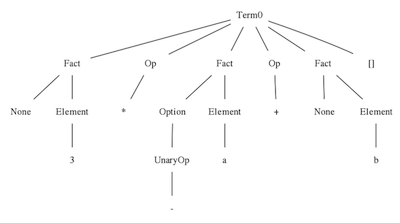
\includegraphics[width=4in]{./examples/ebnf/arith/ebnf-arith.png}
  \caption{Syntax Tree for\\ \textit{3 * -a + b}}
\end{figure}



% EBNF Arith example
\subsection{EBNF - Arith}
This example is similar to the previous two, but we added a few more productions and lexical classes.
We do this by adding unary operations and single length character variables to the grammar definiton. The most important 
differences in this example are the productions that utilize the optional and production ors notion and the
lexical definition that uses the keyword \textit{char}.

The first difference is the optional notation. Below we can see that \textit{unary\_op} is optional because it is
between brackets and anything in between square brackets will be transformed into the OCaml optional type
by gt when generating the parser. \\
%
%
\begin{gt}
Fact : factor -> [ unary_op ] element.
\end{gt}\ \\
%
%
The next major change is the use of vertical bars to denote a type has multiple definitions. This 
can be very useful because it cuts back on defining extra productions. Instead of 
having three different productions for \textit{element} we create one and utilize gt's EBNF notation to define the 
several different possibilities for element.\\
%
%
\begin{gt} 
Element : element -> INT | VAR | LPAREN expr RPAREN.
\end{gt}\ \\
%
%
The last major change is the use of the keyword \textit{char}. If the regular expression for a lexical
definition has a maximum length of one then this keyword is needed. \\
%
%
\begin{gt} 
VAR = char {{ ['a'-'z''A'-'Z']}}.
\end{gt}\ \\
%
%
Gt also supports basic definitions for Emacs and Gedit syntax modes. It is very simple to define basic syntax
modes for the user created language using gt. The first thing the user needs to do is to define a file extensions.
After a file extension is defined the user can map terminals that are not in the abstract syntax tree to
predefined keywords. If the user does not define a syntax mode every terminal that is not in the abstract syntax tree
will be mapped to \textit{keyword} and the file extension will be the \textit{grammar\_name}. \\
\begin{gt}
file_ext = "gra"
keywords = 
	("x","+","-") : special
	(")","(") : keyword
\end{gt} 
%
Below is the whole grammar definition for the \textit{arith} grammar. The file name is \textit{ebnf-example.gra} and it can 
be located in the \textit{gt/tests/ebnf} directory.\\
%
%
\begin{gt}
arith

Term : expr -> factor { op factor }(right,>=0).
Fact : factor -> [ unary_op ] element.
Element : element -> INT | VAR | LPAREN expr RPAREN.

Op : op -> PLUS | TIMES.
UnaryOp : unary_op -> MINUS.

PLUS = "+".
TIMES = "x".
MINUS = "-".
LAPREN = "(" .
RPAREN = ")".
INT = {{ ['0'-'9']+ }}.
VAR = char {{ ['a'-'z''A'-'Z']}}.

file_ext = "gra"
keywords = 
	("x","+","-") : special
	(")","(") : special
\end{gt} 


\subsubsection{Generated Functions}
The files that are generated by gt for this grammar start with \textit{simple}. For example, the equality function
is called \textit{simple\_eq.ml} which is shown below. The equality function takes in a 
pair and returns true if the two elements in the pair are equal otherwise it returns false. The type for the equality 
function is $ ('a * 'a) \rightarrow bool $. \\
\lstinputlisting[language=ML]{./examples/bnf/simple/simple_eq.ml}\ \\
%
%
\noindent Another file that is outputted by gt is the file containing the pretty printer function.
As the name implies, pretty printer helps print the parsed program in a readable format. Instead of
printing out the text that the generated parser has after creating the syntax trees, this function 
preserves the newlines of the original file. However, the pretty printer does not preserve 
comments, tabs or spaces. Below is the pretty printer definition for this example, \textit{simple\_pp.ml}.\\
%
%
\lstinputlisting[language=ML]{./examples/bnf/simple/simple_pp.ml}\ \\
\noindent The following is the output for the function that creates a Graph-Viz file. This function
will create a visual representation of a syntax tree for a program that is parseable by the generated 
parser. \\
\lstinputlisting[language=ML]{./examples/bnf/simple/simple_gviz.ml}

\subsubsection{Syntax Trees}


Now that the parser for the given file has been generated by gt it is ready to be used. 
Figure 2.3 shows the syntax tree that is generated by the above grammar.
%
%
%
\begin{figure}[h!]
  \centering
  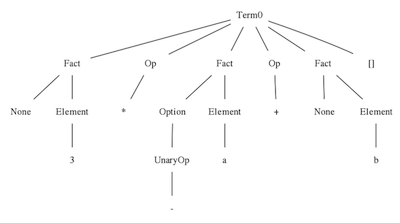
\includegraphics[width=4in]{./examples/ebnf/arith/ebnf-arith.png}
  \caption{Syntax Tree for\\ \textit{3 * -a + b}}
\end{figure}

